\documentclass[twocolumn]{aastex62}

\newcommand{\vdag}{(v)^\dagger}
\newcommand\aastex{AAS\TeX}
\newcommand\latex{La\TeX}
\usepackage{amsmath}
\usepackage{physics}
\usepackage{hyperref}
\usepackage{natbib}
\usepackage[T1]{fontenc}
\usepackage[english]{babel}
\usepackage[utf8]{inputenc}
\usepackage{wasysym}

\begin{document}

\title{\Large AST5220-Milestone I: The Background Cosmology}

\author{Nils-Ole Stutzer}

\begin{abstract}
    We have simulated the large scale evolution of the universe. The expansion
    rate of the universe was computed, by the Friedmann equation, and from it the particle
    horizon scale (the conformal time) and evolution of the matter-energy components of the universe were computed. 
    Having solved for the matter-energy components in the universe we could find in which period each components was dominant. 
    The matter-radiation equality was found to be at log-scale factor
    $x\sim -7$ and the matter-dark energy equality at quite resent times $x\lesssim 0$. The behavior of
    the computed quantities were consistent with known approximations and known results.
\end{abstract}

\section{Introduction} \label{sec:Intro}
In order to describe the universes evolution the first, perhaps most fundamental
part, is to describe its large scale dynamics. Thus in this project we will define 
some concepts and quantities used to describe the
large scale dynamics of the universe as a whole, since the Big Bang until
today. This large scale motion is often called the Background Cosmology. 
The main equation used for this is
the Friedmann equation quantifying the universes expansion rate. From the Friedmann
equation many other interesting quantities can be computed. Furthermore, we will study how the different components
of the matter-energy content of the universe evolves and how the particle horizon
evolves as the universe expands.

\section{Method} \label{sec:Method}
\subsection{Concepts and Quantities}
Before starting on how to solve for the evolution of the universe as a whole, we
start introducing some concepts and quantities.
Because we know from previously conducted cosmological experiments (\cite[Planck Collaboration]{planckcollaboration:2018}) that
the universe is nearly flat, we will here only consider the case of a flat
universe filled with a homogenous and isotropically distributed matter-energy
content. The latter of which is called the cosmological principle. Doing this,
the invariant line-element is given by the Friedmann–Lemaître–Robertson–Walker
metric (FLRW metric) 
\begin{align}
    ds^2 &= -c^2dt^2 + a^2(t)(dr^2 + r^2(d\theta^2 +\sin^2\theta d\phi^2))\\
    & = a^2(t)(-d\eta^2 + dr^2 + r^2(d\theta^2 +\sin^2\theta d\phi^2)),
\end{align}
where $a(t)$ and $eta$ denote the scale factor and the conformal time
respectively. The scale factor quantifies the expansion of the universe, being a
translation factor between proper (physical) and comoving distances. For
convenience we introduce the log-scale factor $x \equiv \log a$ (base $e$),
because we will consider a wide range of universe scales. The universe scale
today at $t = t_0$ is  normalized to $a(t = t_0) = a_0 = 1$, or in log-scale $x_0 = 0$. The
conformal time is the total time a photon is able to travel since the Big Bang
at $t = 0$
until a time $t$, and is thus also a measure of cosmic time. It is thus equivalent to the particle horizon scale of the
universe at any given time, and we will here define it by an ordinary
differential equation (ODE)
\begin{align}
    \dv{\eta}{t} = \dv{\eta}{a}\dv{a}{t} =  \frac{c}{a},
\end{align} 
which we can rewrite into 
\begin{align}
    \dv{\eta}{a} = \frac{c}{a^2 H} = \frac{c}{a\mathcal{H}}.
    \label{eq:conf_time}
\end{align}
Here $H(a)\equiv \frac{\dot{a}}{a}$ is the Hubble parameter measuring the
expansion rate of the universe. We define the scaled Hubble parameter
$\mathcal{H}(a) \equiv aH(a)$. 

The Hubble parameter is given by the Friedmann
equation
\begin{align}
    H = H_0 \sqrt{(\Omega_{b,0} + \Omega_{CDM,0})a^{-3} + \Omega_{r,0} a^{-4} + \Omega_{\Lambda,0}},
    \label{eq:friedmann}
\end{align} 
where $H_0 = 100 h$ $\mathrm{km s^{-1} Mpc^{-1}}$ is the Hubble parameter today
(Hubble constant, and the dimensionless Hubble parameter we here set to $h = 0.7$) and the $\Omega_{x,0}$'s are the matter-energy density parameters
today defined as $\Omega_{x,0}\equiv \frac{\rho_{x,0}}{\rho_{c,0}}$ for a energy
component $x$. The critical density $\rho_c\equiv \frac{3H^2}{8\pi G}$, is the
density needed in order to have a flat universe, and is today equal to
$\rho_{c,0}\equiv\frac{3H_0^2}{8\pi G}$.  

In order to know whether the conformal time is computed right, one can compare it
to the analytical approximations for each epoch of dominance. These are 
\begin{align}
    \eta_r(a) &= \frac{c}{aH} = \frac{c}{\mathcal{H}(a)}\\
    \eta_m(a) &= \eta(a_*) + 2c\left(\frac{1}{\mathcal{H}(a)} - \frac{1}{\mathcal{H}(a_*)}\right)\\
    \eta_\Lambda(a) &= \eta(\tilde{a}) + c\left(\frac{1}{\mathcal{H}(\tilde{a})} - \frac{1}{\mathcal{H}(a)}\right),
\end{align}
for the conformal time in the epoch of dominance for radiation, matter (baryons
+ CDM) and dark matter respectively. Here $a_*$ and $\tilde{a}$ denote the scale
factor when $\Omega_m  = \Omega_b + \Omega_{CDM} \approx 1$ and $\Omega_\Lambda \approx 1$ respectively.

In order to know how much each component of the matter-energy content of the
universe contributes to the total energy content, we can compute the
matter-energy density of each component. This is done when solving the
continuity equation 
\begin{align}
    \dot{\rho} + 3H(\rho + P) = 0,
\end{align}
having the solution 
\begin{align}
    \rho_{x} = \rho_{x,0} a^{-3(1+\omega)},
\end{align}
where $\rho_x$, $\rho_{x,0}$ and $\omega = P/\rho$ are the density at a given
time $a(t)$, the density today and the equation of state (EOS) parameter for a
matter energy component $x$, respectively. For pressure-less fluids like baryons
and cold dark matter (CDM) $\omega = 0$, for relativistic particles like
radiation $\omega = 1/3$ and for dark energy (the cosmological constant) $\omega
= -1$. 

It is, however, more convenient to instead compute the energy density parameters
given as 
$\Omega_x(a) = \rho_x / \rho_c$ at any time, as this is more general. Writing out these we get for a
component $x$ that 
\begin{align}
    \Omega_x &= \frac{\rho_x}{\rho_c} = \frac{\rho_{x,0}a^{-3(1+\omega)} 8\pi G}{3 H^2} \\
   &= \frac{\rho_{x,0}}{\rho_{c,0}/H_0^2} \frac{a^{-3(1+\omega)}}{H^2} \\ 
   &= \frac{\Omega_{x,0}}{(H/H_0)^2} a^{-3(1+\omega)}.
\end{align}

Inserting the respective EOS parameters we get that the energy density parameter
for baryonic matter, CDM, radiation and dark energy ($\Lambda$)
at any given universe scale $a$ is given as

\begin{align}
    \Omega_b(a) &= \frac{\Omega_{b,0}}{a^3 (H/H_0)^2}\\
    \Omega_{CDM}(a) &= \frac{\Omega_{CDM,0}}{a^3 (H/H_0)^2}\\
    \Omega_r(a) &= \frac{\Omega_{r,0}}{a^4 (H/H_0)^2}\\
    \Omega_\Lambda(a) &= \frac{\Omega_{\Lambda,0}}{(H/H_0)^2},
\end{align}
where we have neglected the curvature parameter $\Omega_k$, sometimes included in
the energy-density parameters, as we only consider a flat universe here. Also we
have not included the neutrinos in the calculations. 

We know that at any given time these density parameters must sum to 1, as they
respectively represent the fraction of matter-energy contribution to the total
content of the universe. This can for instance be seen from the Friedmann
equation (\ref{eq:friedmann}), when inserting the scale factor today $a_0 = 1$,
we must recover $H = H_0$ or else it would not make sense. Thus the density
parameters today sum to 1, and for any other time one can simply sum the above
density parameters and check whether they sum to unity.
The values of the density parameters today are well known from cosmological
surveys like Planck, and we will here use the values provided by \cite{callin:2006}. These can be found in Table \ref{tab:params}

\begin{deluxetable}{rc}
	%\tablewidth{0pt}
	\tablecaption{Table showing the energy density parameter values at the current time \cite{callin:2006}. \label{tab:params}}
	%\tablecomments{}
	
	\tablecolumns{2}
	\tablehead{$x$ & $\Omega_{x,0}$}
	\startdata
	$CDM$  &  0.224  \\
	$b$ & $0.046$  \\
	$\Lambda$ & $0.72995$   \\
	$r$ & $5.042\cdot 10^{-5}$  
	\enddata
\end{deluxetable}

Note that the radiation density parameter is given by 
\begin{align}
    \Omega_r = 2\frac{\pi^2}{30} \frac{(k_B T_{CMB})^4}{\hbar^3 + c^5}\frac{8\pi G}{3H_0^2},
\end{align}
where the temperature of the Cosmic Microwave Background (CMB) $T_{CMB} =
2.7255\mathrm{K}$, and the Boltzmann constant, reduced Planck constant and the speed of
light take their regular SI values in our calculations.

\subsection{Implementation}

We want to know how the universe as a whole evolves from the Big Bang until
today. To do that we want to compute the evolution of the regular and the scaled
Hubble parameters as a function of the log-scale factor $x$ (as we consider a wide
range of scales $a$). This is simply done by generating an array of $x$ values
and compute the Hubble parameters from the Friedmann equation
and the scaled Hubble parameter by simply multiplying the
regular Hubble parameter by the scale factor $a = e^x$. One can simply use the
Friedmann equation on the form (\ref{eq:friedmann}), only having to change the
scale factors $a$ to log-scale factors $a = e^x$. Next, one can compute the
density parameters from their definition given in the previous subsection, by
simply also exchanging the scale factor with an exponential of the log-scale
factor. 
\begin{figure*}
    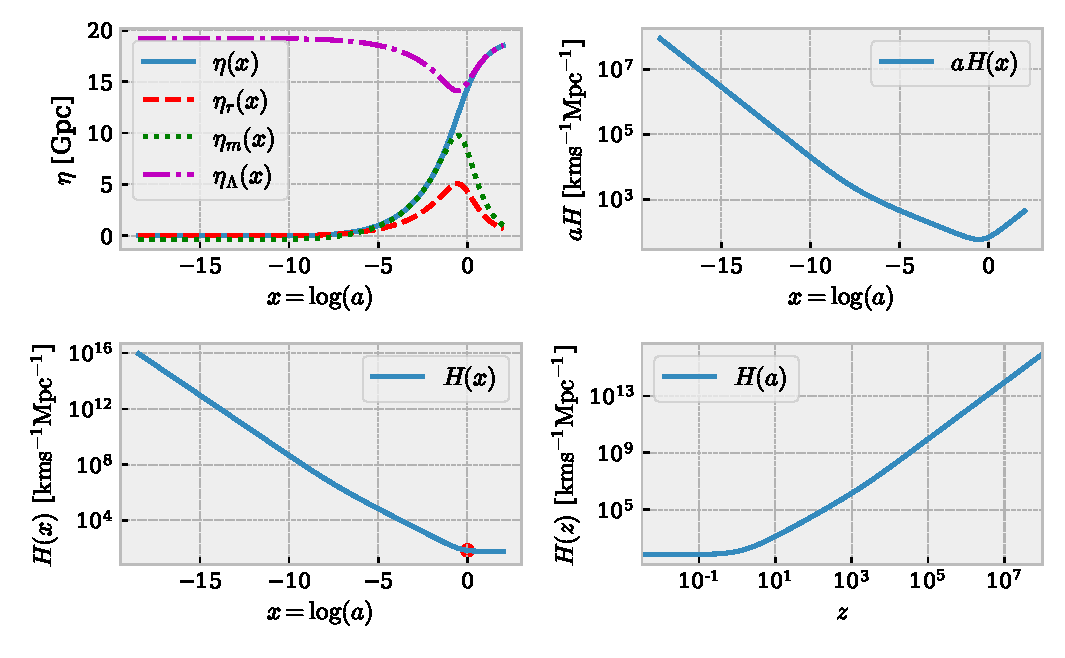
\includegraphics[scale=1]{Figures/Eta_&_H_of_x.pdf}
    \caption{\textbf{Upper left:} The figure shows the conformal time $\eta$(horizon scale) in Gpc as a function of the log-scale factor $x$. Overplotted are the analytical approximations for each era of domination. \textbf{Upper right:} The figure shows the scaled Hubble parameter (expansion rate $\dot{a}$) as a function of the log-scale factor $x$. \textbf{Lower panels:} Here the Hubble parameter $H$ is shown as a function of the log-scale factor $x$ (\textbf{left panel}) and as a function of the scale factor $a$ and the redshift $z$ (\textbf{right panel}), in addition to a red dot illustrating the Hubble parameters value today. Note that the Hubble parameter as a function of the redshift is only plotted from early times until today, while the remaining plots go a bit further.}
    \label{fig:Eta}
\end{figure*}

\begin{figure*}
    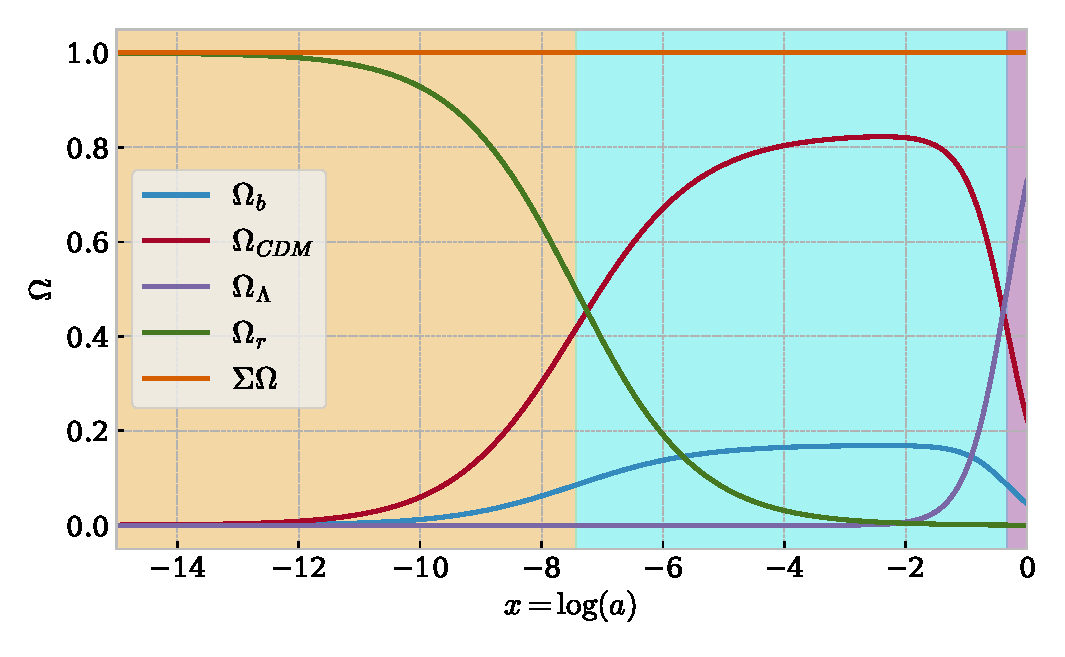
\includegraphics[scale=1]{Figures/Omegas_of_x.pdf}
    \caption{The figure shows the matter-energy density parameters of each component of the total matter-energy content of the universe. Also shown is the sum of all density parameters. To illustrate which component dominates the energy content of the universe at each time, we have colored the radiation dominated era yellow, the matter dominated era blue and the era dominated by dark energy by purple.}
    \label{fig:Omegas}
\end{figure*}

Further, we want to compute the conformal time (particle horizon scale). This is
done by simply solving the ODE given in equation (\ref{eq:conf_time}) using the
\texttt{ODESolver} (C++) module kindly provided by Hans A. Winther. We use initial
conditions $\eta(x) = 0$, as the horizon was very small at early times. We
cannot use $a = 0$ here, though, as this results in a singularity. We thus use
$a = 10^{-8}$, corresponding to $x \approx -18.42$, to represent the scale at
early times being essentially zero. 
After solving for $\eta(x)$ we have a discrete set of conformal times and
corresponding log-scale factors. To get a more continuos representation, we then
perform a cubic spline interpolation, so as to enable computation of the
conformal time between the previously found discrete values. This is done using
the \texttt{Spline} module kindly provided by Hans A. Winther. 
We let the simulation run until $x = 5$ so as to see what happens
beyond the current age. We solve the ODE using 1000 points and save them to a
file together will the corresponding other quantities (the $\Omega$'s, $\mathcal{H}$ etc.). 
Note however, one could save another number of grid points to file, as we made a continuos 
callable spline of the solved data.

To illustrate the evolution of the large scale universe we now plot the
density parameters as a function of the log-scale factor $x$, as well as the
horizon scale, the regular and scaled Hubble parameters as functions of $x$.
Also we plot the Hubble parameter as a function of redshift $z$, being another
measure of time. It is related to the scale factor by $a^{-1} = 1 + z$, and
measures how much a wavelength of light is stretched as light travels through an
expanding universe.

Furthermore, we implemented functions computing the first and second order derivatives of the
scaled Hubble parameter. This was done in order to make further extensions to the program easier. 
The first derivative was found to be 
\begin{align}
    \mathcal{H}' = \dv{(e^x H)}{x} = \frac{H_0^2}{2\mathcal{H}}\sum_i \Omega_i (2-b_i)e^{(2-b_i)x},
\end{align}
by simply differentiating $\mathcal{H} = aH = e^xH$, for the sum over all matter-energy components $i$. 
Here $b_i = -3(1 + \omega_i)$ for an EOS parameter $\omega_i$. The second order derivative is simply found by again
differentiating the above expression. We found the second order derivative to be 
\begin{align}
    \mathcal{H}'' &= \frac{H_0^2}{2\mathcal{H}^2}\sum_i(2-b_i)^2\Omega_i e^{(2-b_i)x}\\ 
    &- \frac{H_0^4}{4\mathcal{H}^3}\left(\sum_i(2-b_i)\Omega_i e^{(2-b_i)x}\right).
\end{align}
We found that the ratios $\mathcal{H}' / \mathcal{H} = (1 - b_i / 2)$ and $\mathcal{H}'' / \mathcal{H} = \frac{1}{4}(2 - b_i)^2$, which is a convenient relation for debugging the code.

\section{Results/Discussion}\label{sec:Results}
When running the program we measured a run time of $\sim 10^{-3}$ seconds. Thus a later extensive iterative use
of the solver is enabled, as it takes virtually no time to run the script one single time.

The conformal time (horizon scale) as well as the Hubble
and scaled Hubble parameters as functions of $x$ ($z$ and $a$) can be seen in
Figure \ref{fig:Eta}. As one can see the horizon scale stays very small for a
long while, from early times until $x \approx -7$, then starting to grow
exponentially and finally starting to flatten out towards the end of the
simulated period at around $x\sim 0$. Also we have overplotted the analytical approximations for
conformal time in each of the epochs of dominance to check whether our solution
to the conformal time makes sense. See Appendix A for derivation of the
approximations. We see that the approximations overlap the conformal time
resonantly well withing their respective intervals of validity. The reason the horizon scale flattens out 
in the dark energy epoch is probably due to an Einstein-de Sitter (EdS), i.e. dominated by dark energy, does not have a particle horizon. 
This is easily seen when solving for $\eta$. Therefore the particle horizon, i.e. the limit to where one can see, is set to its
maximum extension in the previous epoch (the matter dominated epoch). 

The expansion rate quantified by the scaled Hubble parameter $\mathcal{H}(x) =
aH(x)$ is also seen in Figure \ref{fig:Eta}. We can clearly see from its shape
in which era of the universe we are in. At early times, when the universe was
radiation dominated the scaled Hubble parameter $\mathcal{H} \propto a^{-1}$.
When matter (baryons and CDM) eventually started dominating, the expansion rate
scaled differently; $\mathcal{H}\propto a^{-0.5}$, having a somewhat shallower
slope compared to the expansion rate at radiation dominance. We can clearly see these theoretical slopes indeed appear in the plot.
This transition
seems to happen at $x\sim -7$, coinciding roughly with the sudden growth of
$\eta$, as seen for the change in slope of $\mathcal{H}$. Finally we see the
transition from a decelerating universe, to an accelerating one. The expanding
universe halts, as seen by the extremum of $\mathcal{H}$, after which the curve
turns upwards. This corresponds to the era of dark matter, where the universe
gradually turns to an exponential expansion rate, as seen by the linearly rising scaled Hubble parameter past the current time.
This is when the universe starts to behave like an 
EdS universe dominated by dark energy and expanding exponentially.
This era started quite recently at $x\lesssim 0$. The hypothesis that dark energy now dominates the universe is further
supported by the fact that the regular Hubble parameter seen in the bottom left
panel of Figure \ref{fig:Eta} becomes almost constant (in the log-log) after
crossing into the era of dark energy. This is also easily seen from the Friedmann
equation becoming constant in this epoch, assuming that the other density parameters are negligible. Another
noteworthy thing is that the Hubble parameter seems to hit its known current
value (see red dot in Figure \ref{fig:Eta}) pretty well, putting further
evidence on that the solving of the equations are done correctly. The plot in the lower right
panel of Figure \ref{fig:Eta} tells the same story as the lower left one,
however, it is nice to see the redshift dependence of the Hubble
parameter directly as a comparison.

The evolution of the density parameters is shown in Figure \ref{fig:Omegas} and effectively
illustrates at which point each of the components dominate, to a more direct degree as in Figure \ref{fig:Eta}. 
We see as expected
that at any given time the density parameters sum to unity. At early times the
universe was dominated by radiation as seen by the fact that $\Omega_r \approx
1$. This epoch is marked by a yellow background. Then when the matter starts to
dominate, i.e. $\Omega_B + \Omega_{CDM} \approx 1$, we see a gradually
decelerating radiation contribution. This is marked by a blue background. The
epoch accelerating expansion of the universe when dark energy dominates is
marked by a purple background. Note that the transitions between one to another
epoch of dominance is not sharp, but rather a smooth transition, something
which is not illustrated here by the background color. Also noteworthy is that the approximate time
(scale) of transition between each era seems to coincide well with the time of
transition earlier discussed, supporting the notion that one can estimate the 
era of dominance by the behavior of the quantities in Figure \ref{fig:Eta}. 

All in all we seem to recover results consistent
with known science and approximations. We can thus justify a conclusion that the 
simulations are significant results.


\section{Conclusion} \label{sec:Conclusion}
We have simulated the large scale motion of the universe as a whole, and seen
how the expansion rate and particle horizon scale of the universe is affected by
the different matter-energy contributions contained within the universe. Also
the evolution of the matter-energy contribution of each component was simulated.
The results of the simulations where found to be consistent with known
approximations and known results, therefore justifying the conclusion that the
results are significant.


\bibliography{ref}
\bibliographystyle{aasjournal}

\section{Appendix A} \label{apx:A}
When within the epoch of radiation dominance we can from the Friedmann equation
see that the Hubble parameter
\begin{align}
    H^2 = H_0^2 \frac{\Omega_{r,0}}{a^4}.
\end{align}
The conformal time then becomes simplified making it 
\begin{align}
    \eta_r(a) = \int_0^a \frac{c da}{a^2 H(a)} \approx \int_0^a\frac{c da}{a^2 H_0 \sqrt{\Omega_r}}a^2 = \frac{ca}{H_0\sqrt{\Omega_r}} = \frac{c}{aH} = \frac{c}{\mathcal{H}(a)}. 
\end{align}
This expression is valid for $\Omega_r(a) \approx 1$. At scales $a_*$ where $\Omega_m(a_*)\approx
1$, where $\Omega_m = \Omega_B + \Omega_{CDM}$ we have a similar approximation
\begin{align}
    \eta_m(a) &= \eta(a_*) + \int_{a_*}^a \frac{cda}{a^2H} \approx \eta(a_*) + \int_{a_*}^a \frac{cda}{a^2H_0\sqrt{\Omega_m}}a^{3/2} = \eta(a_*) + \int_{a_*}^a \frac{da}{\sqrt{a}} \\
    &= \eta(a_*) + 2c\left(\frac{1}{aH} - \frac{1}{a_*H(a_*)}\right) = \eta(a_*) + 2c\left(\frac{1}{\mathcal{H}(a)} - \frac{1}{\mathcal{H}(a_*)}\right).
\end{align}
Here $\eta(a_*)$ is the conformal time when matter domination starts. Note that
since we looked at the matter dominated era, we could use the Friedmann
equation on the form 
\begin{align}
    H^2 = H_0^2 \frac{\Omega_m}{a^3}.
\end{align}
Finally we can also consider the case where the matter-energy is dominated by
dark energy at $\tilde{a}$ so that $\Omega_\Lambda(\tilde{a})\approx 1$. Then we
can write 
\begin{align}
    H^2 = H_0 \Omega_\Lambda, 
\end{align}
enabeling us to write 
\begin{align}
    \eta_\Lambda(a) &= \eta(\tilde{a}) + \int_{\tilde{a}}^a\frac{cda}{aH} = \eta(\tilde{a}) + \frac{c}{H_0\sqrt{\Omega_\Lambda}}\int_{\tilde{a}}^a\frac{da}{a^2} \\
    &= \eta(\tilde{a}) + c\left(\frac{1}{\mathcal{H}(\tilde{a})} - \frac{1}{\mathcal{H}(a)}\right).
\end{align}
Here we let $\eta(\tilde{a})$ denote the conformal time when the dark energy
dominated era started. These three expressions can now be used to check whether
the full computed conformal time is reasonable.

\section{Appendix B} \label{apx:B}
In order to check whether we implemented $\mathcal{H}'$ and $\mathcal{H}''$ correctly we 
plotted the ratios of these to the undifferentiated scaled Hubble parameter. This gave us 
the plots seen in Figure \ref{fig:derivatives}. As seen the ratio $\mathcal{H}' / \mathcal{H}$
reaches the wanted constant value in each of the three epochs of dominance. Similarly,
for the ratio $\mathcal{H}''/ \mathcal{H}$ we see that the radiation and dark energy dominated
eras, the ratio reaches the same value (equal to one) and that the ratio in the matter dominated
era almost reaches its expected ratio value. This justifies the conclusion that the first and second
order derivatives of $\mathcal{H}$ were in fact implemented correctly, since we recover the 
expected behavior within each of the epochs.

\begin{figure*}
    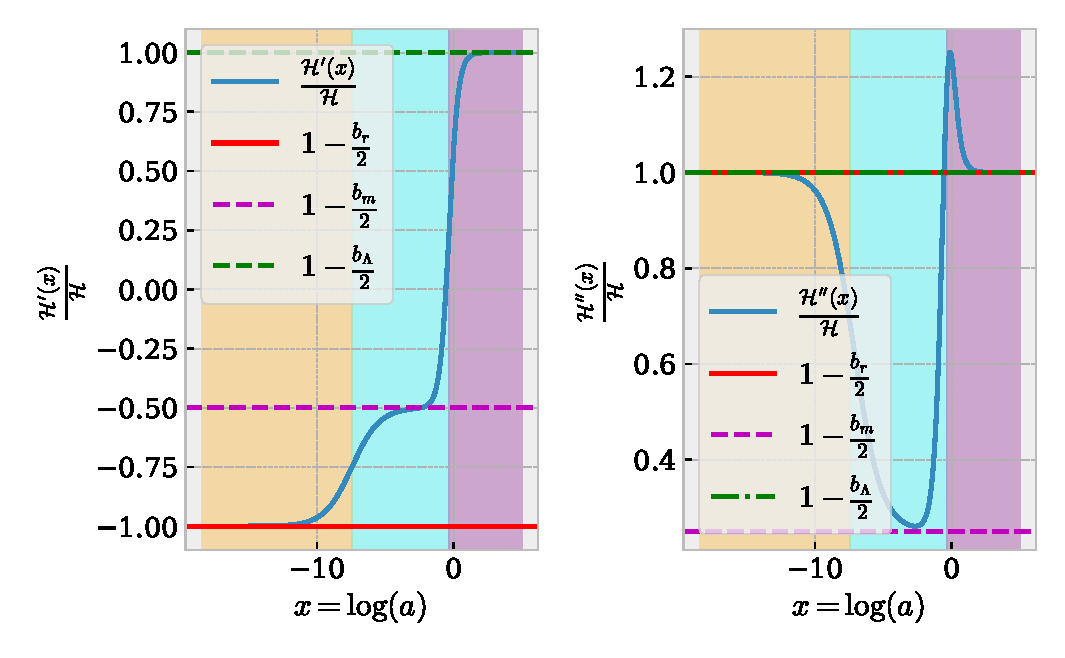
\includegraphics[scale=1]{Figures/derivatives.pdf}
    \caption{\textbf{Upper left:} The figure shows the first and second derivative
    of the scaled Hubble parameter divided by it, i.e. $\mathcal{H}'/\mathcal{H}$ and $\mathcal{H}'' / \mathcal{H}$.
    Also plotted are the respective constant values, indicated by dashed lines, 
    that should be reached within each regime of dominance.}
    \label{fig:derivatives}
\end{figure*}

\end{document}